% \documentclass[preprint]{aastex}
%\documentclass{article}
\documentclass{report}
\usepackage{graphicx}
\usepackage{subfigure}
\usepackage{rotating}
\usepackage{lscape}
\usepackage{natbib}
\usepackage{hyperref}
\pagestyle{empty}
\usepackage{aas_macros}
\usepackage{longtable}
\usepackage{amsmath}
\bibliographystyle{apj}

\hypersetup{
  bookmarks=true,         % show bookmarks bar?
  unicode=false,          % non-Latin characters in Acrobat's bookmarks
  pdftoolbar=true,        % show Acrobat's toolbar?
  pdfmenubar=true,        % show Acrobat's menu?
  pdffitwindow=true,      % page fit to window when opened
  pdftitle={Stellar Locus Regression Manual},    % title
  pdfauthor={F. William High},     % author
  pdfsubject={astronomical calibration},   % subject of the document
  pdfnewwindow=true,      % links in new window
  pdfkeywords={astronomy, colors, calibration, stars}, % list of keywords
  colorlinks=true,        % false: boxed links; true: colored links
  linkcolor=red,          % color of internal links
  citecolor=red,          % color of links to bibliography
  filecolor=magenta,      % color of file links
  urlcolor=blue           % color of external links
}

\newcommand{\zptcolor}{\boldsymbol{\kappa}}
%\newcommand{\atmextcolor}{\mathcal{E}^{\text{A}}}
%\newcommand{\galextcolor}{\mathcal{E}^{\text{G}}}
\newcommand{\atmextcolor}{\boldsymbol{E}^{\text{A}}}
\newcommand{\galextcolor}{\mathcal{E}^{\text{G}}}
%\newcommand{\color}{\mathcal{C}}
\newcommand{\color}{\boldsymbol{c}}
%\newcommand{\colormatrix}{\mathcal{M}}
\newcommand{\colormatrix}{\mathbf{B}}
\newcommand{\identity}{\boldsymbol{1}}
\newcommand{\colorairmassmatrix}{\mathbf{T}}
\newcommand{\sdss}{SDSS}
\newcommand{\slr}{SLR} 
\newcommand{\imacs}{IMACS}
\newcommand{\ldss}{LDSS3}
\newcommand{\tmass}{2MASS}
\newcommand{\reflex}{REFLEX}
\newcommand{\gof}{GOF} 
\newcommand{\ndeg}{{$^{\circ}$}}
\newcommand{\metal}{[\text{Fe}/\text{H}]}

\begin{document}

\title{Stellar Locus Regression\\User Manual}

\author{F.\ William High}

\date{\today}


\pagenumbering{roman}

%% Personalized Title Page
\begin{titlepage}
\begin{minipage}{\textwidth}
\begin{center}
\Huge
Stellar Locus Regression\\User Manual\\
\vspace{3cm}
\Large
F.~William High\\
\vspace{3cm}
\large
Department of Physics\\ Harvard
University\\ 17 Oxford Street\\ Cambridge, MA 02138\\
\href{mailto:high@physics.harvard.edu}{high@physics.harvard.edu}\\
\url{http://physics.harvard.edu/~high}
\end{center}
\end{minipage}
\end{titlepage}

\begin{minipage}{\textwidth}

\section*{}

Copyright \copyright{}  2009  Fredrick William High.\\
Permission is granted to copy, distribute and/or modify this document
under the terms of the GNU Free Documentation License, Version 1.3
or any later version published by the Free Software Foundation;
with no Invariant Sections, no Front-Cover Texts, and no Back-Cover Texts.
A copy of the license is included in the section entitled "GNU
Free Documentation License".

% \section*{Acknowledgements}

% Stellar Locus Regression was developed with Christopher Stubbs, Armin
% Rest, Brian Stalder, and Pete Challis at Harvard University.  Thanks
% to Patrick Kelly, for useful conversations.

\end{minipage}

% \begin{abstract}

%   Stellar Locus Regression (\slr) is an algorithm that takes
%   uncalibrated astronomical magnitudes of stars from any field and
%   calibrates the colors, which are magnitude differences, without the
%   traditional use of standard stars. \slr\ exploits the fact that the
%   majority of stars in the sky have colors that occupy a well defined,
%   nearly one-dimensional region in hyperdimensional color-color
%   space. This is called the stellar locus. \slr\ regresses raw colors
%   to a standard stellar locus, delivering best-fit calibration terms,
%   which can be applied to the other point- and extended-sources in the
%   catalog. \slr\ can be performed on as few as 7 stars and in fields of
%   view down to 8 arcminutes. \slr\ can be performed in real time,
%   during observation.

%   This is a short guide to installing and running the stellar locus
%   regression (\slr) on example and user data.  A more detailed
%   description of the \slr\ alogrithm and verifcation of its
%   effectiveness is available, see \citet{bib:slr}.  Since this is an
%   evolving code, this guide will supercede the paper if there are
%   differences.

% \end{abstract}


\tableofcontents
\pagenumbering{arabic}
\setcounter{page}{1}

% \input{preliminaries}

\chapter{Introduction}

Stellar Locus Regression (\slr) is a method of directly adjusting the
instrumental broadband optical colors of stars to bring them into
accord with a universal stellar color-color locus, producing
accurately calibrated colors for both stars and galaxies.  This is
achieved without first establishing individual zeropoints for each
passband, and can be performed in real-time at the telescope.  In
\citet{bib:slr} the authors demonstrated how \slr\ naturally makes one
wholesale correction for differences in instrumental response, for
atmospheric transparency, for atmospheric extinction, and for Galactic
extinction.  We are offering open-source access to our IDL routines,
validated and verified for the implementation of this technique.

Figure \ref{fig:algorithm} schematically outlines the technique and
Figure \ref{fig:example} shows the effect of using \slr\ on
uncalibrated data.  The core IDL tools we have developed are available
at \url{http://stellar-locus-regression.googlecode.com}.

\begin{figure}
\center
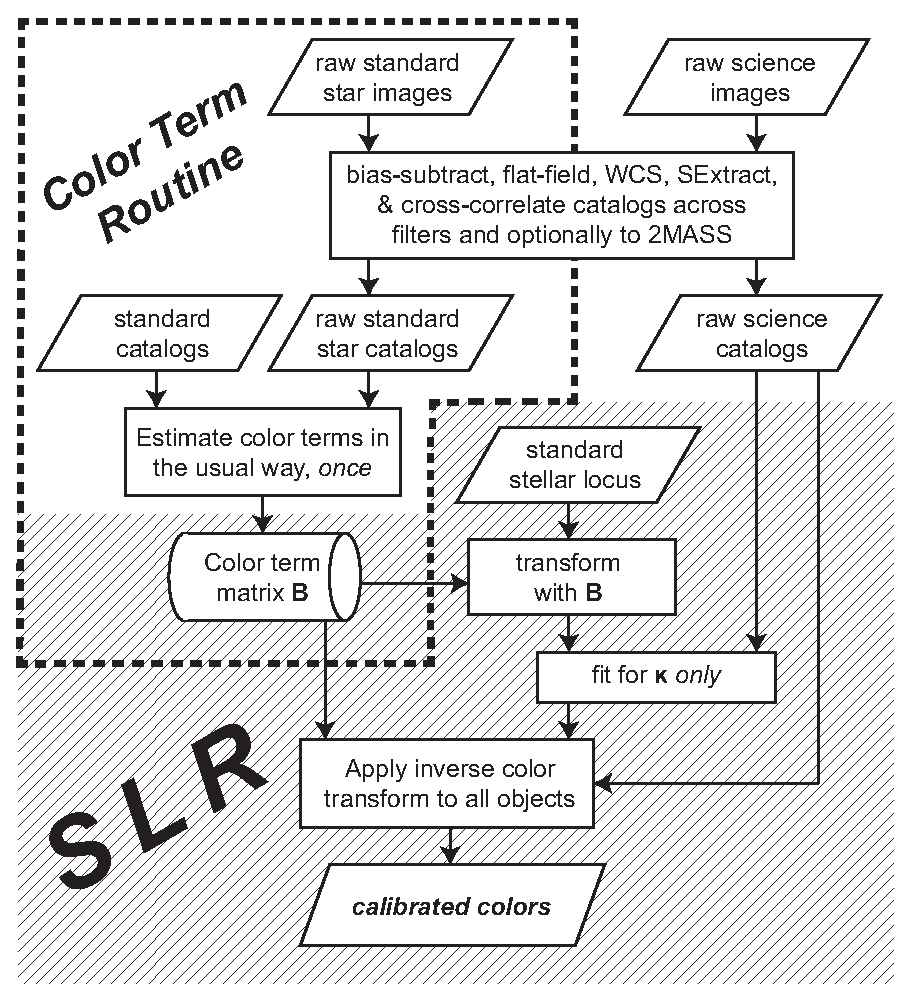
\includegraphics[scale=0.9]{fig/slr_algorithm.eps}
\caption{ \slr\ flow chart for calibrating colors.  The hashed region
  denotes parts of the algorithm that are unique to \slr, while the
  non-shaded region shows steps that are more traditional.  The dotted
  region denotes the color term estimation routine, which need only be
  performed once per detector. }
\label{fig:algorithm}
\end{figure}

\begin{figure}
% \epsscale{0.75}
  \center
 \includegraphics[scale=0.6]{fig/illus_sptcl2332_5051_locus_threepanel.eps}
 \caption{ An illustration of Stellar Locus Regression (\slr).  Colors
   are plotted on the SDSS photometric system. All panels show the
   standard stellar locus (black line and gray density contours),
   reproduced from \citet{bib:covey}.  Red points are stellar colors
   obtained from a Source Extractor analysis of flat-fielded Magellan
   $6.5\,\mathrm{m}$ IMACS images.  {\it Top panels:} The instrumental
   IMACS colors are plotted, with a clear mismatch between them and
   the standard locus. {\it Middle panels:} \slr\ is performed with
   only a common translation vector applied to the instrumental
   colors.  Note the color-dependent discrepancies in the upper right
   portions of the central panels.  By way of example, the vectors
   show the expected direction and magnitude of extinction by Galactic
   dust ($A_r=0.2$) and the atmosphere ($1.3$ airmasses).  {\it Bottom
     panels:} Color terms are measured from a single observation of a
   field containing standard stars. Fixing these color terms, a new
   best-fit translation is determined, which brings the observed
   colors onto the \sdss-calibrated color system, as defined by the
   stellar locus.  This \slr\ analysis, when the corrections are then
   applied to all objects in the photometric catalog, allows us to
   rapidly obtain highly accurate colors on the SDSS system, directly
   from flat-fielded data, with a single correction step that accounts
   for atmospheric extinction, Galactic extinction and instrumental
   response differences.}
 \label{fig:example}
 \end{figure}
%\epsscale{1.0}


\chapter{Quick Start}


\begin{enumerate}
\item \href{http://stellar-locus-regression.googlecode.com}{Download}
  the \slr\ code.
\item Install and set up the \href{http://idlastro.gsfc.nasa.gov}{Goddard
    astronomy} IDL libraries,
  \href{http://www.astro.princeton.edu/~schlegel/code.html}{idlutils},
  and the \href{http://www.physics.wisc.edu/~craigm/idl}{Markwardt IDL
    libraries}.
%\item {\bf Optional:}
%  \href{http://astro.berkeley.edu/~marc/dust}{Install and set up} the
%  \citet{bib:sfd} $E(B-V)$ dust maps and IDL utilities.
\item
  \href{http://www.cfa.harvard.edu/~kcovey/research/medianlocus.tbl}{Download}
  the stellar locus data of \citet{bib:covey} and put them in a
  directory $<$data-dir$>$/covey.
\item Set environment variables (here in tcsh):
\begin{verbatim}
% setenv SLR_INSTALL <install-dir>/slr-v2.1
% setenv SLR_DATA <data-dir>
% setenv PATH {$PATH}:$SLR_INSTALL/bin
\end{verbatim}
\item Verify your installation (see \S\ref{sec:verify}):
\begin{verbatim}
% cd $SLR_INSTALL/example_data
% slr.csh low_reddening.ctab low_reddening.slr.ctab
% slr.csh high_reddening.ctab high_reddening.slr.ctab
% idl
IDL> slr_demo
IDL> slr_docs
\end{verbatim}
\end{enumerate}


\chapter{Installation}

\section{Download}

First, go get the latest version 2 download at
\url{http://stellar-locus-regression.googlecode.com}. Untar
it with
\begin{verbatim}
tar xzvf slr-v2.1.tar.gz
\end{verbatim}
Put the package in some directory $<$install-dir$>$. This can be
/usr/local/idllibraries or \$HOME or whatever you prefer. The
package root directory will then be $<$install-dir$>$/slr-v2.1.

Version 2.1 and higher require only IDL, and do not require
Analyst. Version 2.0 and prior require IDL with the Analyst add-on,
which costs extra.


\section{IDL Libraries}

You'll need these idl libraries:

\begin{enumerate}
\item idlutils from
  \url{http://www.astro.princeton.edu/~schlegel/code.html}.  Any
  installation procedure will do, but you probably want the latest
  idlutils tar file, e.g.\ idlutils-v5\_3\_0.tar.
\item {\it The latest} Goddard astro libraries from
  \url{http://idlastro.gsfc.nasa.gov}.  Note that idlutils comes with
  an old version of the Goddard libraries that is {\it incompatible
    with this implementation of SLR}.  Get the latest one.
\item Markwardt libraries from
  \url{http://www.physics.wisc.edu/~craigm/idl}.  You want
  cmtotal.tar.gz.
\end{enumerate}

Put them in your typical IDL directory. For example, use a directory
you can remember $<$pro-dir$>$, like /usr/local/idllibraries.

Don't forget to add them to your IDL\_PATH with shell startup file
entries similar to:
\begin{verbatim}
% export IDL_PATH=$IDL_PATH:+<pro-dir>/idlutils:+<pro-dir>/markwardt
\end{verbatim}
in bash or
\begin{verbatim}
% setenv IDL_PATH {$IDL_PATH}:+<pro-dir>/idlutils:+<pro-dir>/markwardt
\end{verbatim}
in tcsh.

Of course all of this assumes you have properly initialized the
IDL\_PATH, for example in tcsh:
\begin{verbatim}
% setenv IDL_BIN /usr/local/itt/idl/bin
% source $IDL_BIN/idl_setup
% setenv IDL_PATH <IDL_DEFAULT>
\end{verbatim}

% \section{Optional: Galactic Dust Maps}

% Some optional functionality of \slr\ requires the dust maps of
% \citet{bib:sfd}.  To enable these functions, the maps need to be
% located in \$DUST\_DIR/maps. Here's how to set this up:

% Go to \url{http://astro.berkeley.edu/~marc/dust} to get the dust maps
% and IDL code.

% Follow their install instructions. You only need the high resolution
% 4096 $E(B-V)$ maps, both the north and south Galactic planes (NGP and
% SGP). Put them in some directory, for example
% $<$install-dir$>$/slr-v2.2/example\_data/sfd/maps. Make sure the top
% directory is maps and not map. Put the SFD IDL code in some
% $<$pro-dir$>$ and add to IDL\_PATH.

% As instructed at the website, set the DUST\_DIR environment
% variable. If you used our suggestion, then you would issue
% \begin{verbatim}
% % setenv DUST_DIR <install-dir>/slr-v2.1/example_data/sfd
% \end{verbatim}

% The directory \$DUST\_DIR/maps must exist and contain the E(B-V)
% dust maps.

\section{Standard Stellar Locus}

\slr\ gets the standard stellar locus data from the directory
\$SLR\_DATA/covey.

Go get Kevin Covey's stellar locus data, which he makes available on
his own website. You'll need the stellar data\\
\url{http://www.cfa.harvard.edu/~kcovey/research/superclean.fits}\\
and the median locus line data:\\
\url{http://www.cfa.harvard.edu/~kcovey/research/medianlocus.tbl}\\
Put them in some directory $<$data-dir$>$/covey. We suggest putting
them in the $<$install-dir$>$/example\_data/covey subdirectory of
your installation. Set SLR\_DATA. If you used our suggestion, then
you would issue

\begin{verbatim}
% setenv SLR_DATA <install-dir>/example_data
\end{verbatim}

The directory \$SLR\_DATA/covey must exist and contain
medianlocus.tbl and superclean.fits.

\section{Environment Variables}

Now set some environment variables in your cshrc or bashrc file. Remember to insert the appropriate directories. Example is for tcsh:
\begin{verbatim}
% setenv SLR_INSTALL <install-dir>/slr-v1.0
% setenv SLR_DATA <data-dir>
% setenv IDL_PATH {$IDL_PATH}:+$SLR_INSTALL/pro
% setenv PATH {$PATH}:SLR_INSTALL/bin
\end{verbatim}

We've used the example directories mentioned in this install file. This should let the demo (see below) work properly. If you made different choices, you must make sure these environment variables reflect them.

\section{Verifying Your Installation}
\label{sec:verify}

If everything is set up properly, you can run the demo by invoking idl and running:
\begin{verbatim}
% cd $SLR_INSTALL/example_Data
% idl
IDL> slr_demo
\end{verbatim}

The first time you run it, it will take some time (it's reformatting
the data to an optimal, IDL-friendly format). It will be faster the
second time.

The demo will run \slr\ on the example Sloan Digital Sky Survey data
that comes with your installation. You should see plots of the stellar
locus (you must hit enter to continue), a visualization of the
numerical regression, and results for best-fit parameters printed to
screen.


\subsection{Running slr.csh Using Example Data}

Go to the directory \$SLR\_INSTALL/example\_data, then issue at
the commandline (you have to be in same directory as your input file):
\begin{verbatim}
% cd $SLR_INSTALL/example_data
% slr.csh low_reddening.ctab low_reddening.slr.ctab
\end{verbatim}

This will run \slr\ on the example colortable we provided (first
argument), and output \slr\ calibrations to another colortable (second
argument). The output colortable is equal to the input colortable but
with the additional appended columns GR, RI, etc, which are the
calibrated colors g - r, r - i. Estimated color errors, with bootstrap
errors added in quadrature, are also output.

Browse the log file that \slr\ generates, in this case
lowext\_stars3\_fwhigh.slr. This contains the color calibrations
with bootstrap errors.

If that works then you should also be able to run
\begin{verbatim}
% cd $SLR_INSTALL/example_data
% slr.csh high_reddening.ctab high_reddening.slr.ctab
\end{verbatim}


\subsection{Running slr.csh with Your Own Data}

To run \slr\ on your own data, issue the command (again, in the same
directory as your input file):
\begin{verbatim}
% slr.csh input.ctab output.slr.ctab <config-file>
\end{verbatim}
The configuration file can optionally be specified.  If none is given,
then the default file is used, \$SLR\_INSTALL/config/default.config.

This has the same output as the previous section.  The requirements
for the input file are as follows:

\begin{enumerate}

\item The first line is a description of the columns followed by a
  $\#$ for example:
\begin{verbatim}
# ID RA Dec type tmixed g g_err r r_err i i_err z z_err ...
\end{verbatim}
  where the ellipsis ... means there are more acceptable columns you
  can specify.  See \S\ref{sec:colortable} for a full description of
  the ``colortable''.
\end{enumerate}




\chapter{Conventions}

Define mathematical conventions.

Assumptions.

Glossary of terms.


\chapter{The Colortable}
\label{sec:colortable}

SLR reads data from and outputs results to what we call {\it
  colortables}.  These are simple ascii files with a single header
that starts with \verb|#| and one row of data per object.  The header
values are columns names, and each row corresponds to one object.  Here's a simple (truncated) example:
\begin{verbatim}
# ID        RA       Dec type tmixed       g  g_err       r  r_err ...
   0 254.00649  34.33696    1      0  20.672  0.025  19.795  0.018 ...
   1 254.05269  34.36260    1      0  16.426  0.004  15.849  0.004 ...
   2 254.02026  34.34031    1      0  23.670  0.283  21.607  0.072 ...
   3 254.00436  34.36294    1      0  20.381  0.021  19.012  0.011 ...
   4 254.02655  34.34580    1      0  18.203  0.006  17.059  0.005 ...
...
\end{verbatim}
The ellipses ... here mean there can be additional columns and rows.

The data must be fixed width.  The header strings however need not be
fixed width.  Empty or erroneous data must generically be represented
by the character ``\verb|-|'' (dash).

While there is a minimal subset of columns that must be present for
SLR to work properly, it is acceptable for there to be extra columns
that the code doesn't formally recognize or use.  This way you can
carry extra information in the colortable, such as \verb|ID| in the
example above.

Table \ref{tab:colortable} lists the columns that are recognized and
used by the SLR code.

\begin{center}
\begin{longtable}{lllcp{2in}}
\caption[Colortable columns.]{Colortable columns.}
\label{tab:colortable} \\
  \hline \hline \\[-2ex]
  \multicolumn{1}{c}{Column name} &
  \multicolumn{1}{c}{Type} &
  \multicolumn{1}{c}{Unit} &
  \multicolumn{1}{c}{Required?} &
  \multicolumn{1}{c}{Description} \\[0.5ex] \hline
\endfirsthead
\multicolumn{5}{c}{{\tablename} \thetable{} continued: Colortable columns.} \\[0.5ex]
  \hline \hline \\[-2ex]
  \multicolumn{1}{c}{Column name} &
  \multicolumn{1}{c}{Type} &
  \multicolumn{1}{c}{Unit} &
  \multicolumn{1}{c}{Required?} &
  \multicolumn{1}{c}{Description} 
\\[0.5ex] \hline
  \\[-1.8ex]
\endhead
\multicolumn{5}{l}{{{\it Continued on next page}\ldots}} \\
\endfoot
  \\[-1.8ex] \hline \hline
\endlastfoot
\verb|ID| & {\it string} & J2000 $\deg$ & Yes & Object identifier. \\
\verb|RA| & {\it float} & J2000 $\deg$ & Yes & Right ascension. \\
\verb|Dec| & {\it float} & J2000 $\deg$ & Yes & Declination. \\
\verb|type| & {\it integer} & & Yes & $1=\textrm{star}$, $3=\textrm{galaxy}$. \\
\verb|tmixed| & {\it boolean} & & Yes & Is the \verb|type| ambiguous between the bands? \\
\verb|U| & {\it float} & mag & No & $U$-band magnitude. \\
\verb|U_err| & {\it float} & mag & If \verb|U| present & Uncertainty in Johnson $U$-band magnitude. \\
\verb|B| & {\it float} & mag & No & $B$-band magnitude. \\
\verb|B_err| & {\it float} & mag & If \verb|B| present & Uncertainty in Johnson $B$-band magnitude. \\
\verb|V| & {\it float} & mag & No & $V$-band magnitude. \\
\verb|V_err| & {\it float} & mag & If \verb|V| present & Uncertainty in Johnson $V$-band magnitude. \\
\verb|R| & {\it float} & mag & No & $R$-band magnitude. \\
\verb|R_err| & {\it float} & mag & If \verb|R| present & Uncertainty in Johnson $R$-band magnitude. \\
\verb|I| & {\it float} & mag & No & $I$-band magnitude. \\
\verb|I_err| & {\it float} & mag & If \verb|I| present & Uncertainty in Johnson $I$-band magnitude. \\
\verb|u| & {\it float} & mag & No & $u$-band magnitude. \\
\verb|u_err| & {\it float} & mag & If \verb|u| present & Uncertainty in SDSS $u$-band magnitude. \\
\verb|g| & {\it float} & mag & No & $g$-band magnitude. \\
\verb|g_err| & {\it float} & mag & If \verb|g| present & Uncertainty in SDSS $g$-band magnitude. \\
\verb|r| & {\it float} & mag & No & $r$-band magnitude. \\
\verb|r_err| & {\it float} & mag & If \verb|r| present & Uncertainty in SDSS $r$-band magnitude. \\
\verb|i| & {\it float} & mag & No & $i$-band magnitude. \\
\verb|i_err| & {\it float} & mag & If \verb|i| present & Uncertainty in SDSS $i$-band magnitude. \\
\verb|z| & {\it float} & mag & No & $z$-band magnitude. \\
\verb|z_err| & {\it float} & mag & If \verb|z| present & Uncertainty in SDSS $z$-band magnitude. \\
\verb|J| & {\it float} & mag & No & $J$-band magnitude. \\
\verb|J_err| & {\it float} & mag & If \verb|J| present & Uncertainty in SDSS $J$-band magnitude. \\
\verb|H| & {\it float} & mag & No & $H$-band magnitude. \\
\verb|H_err| & {\it float} & mag & If \verb|H| present & Uncertainty in SDSS $H$-band magnitude. \\
\verb|K| & {\it float} & mag & No & $K$-band magnitude. \\
\verb|K_err| & {\it float} & mag & If \verb|K| present & Uncertainty in SDSS $K$-band magnitude. \\
\end{longtable}
\end{center}


\chapter{Configuration Parameters}

SLR reads ascii configuration files that the user can edit.  Comments
can be used with the character \verb|#|.  There must be at least one
space between the paramter name and its value.  Arrays (vectors) are
comma-separated lists; there must be no spaces in such lists.  Each
parameter in the config file must have a corresponding value next to
it.  There can be no empty fields.  All parameters must be present in
the file.

Table \ref{tab:config} describes all configuration paramaters.

\begin{center}
\begin{longtable}{llp{2in}}
\caption[Configuration parameters.]{Configuration parameters.}
\label{tab:config} \\
  \hline \hline \\[-2ex]
  \multicolumn{1}{c}{Parameter} &
  \multicolumn{1}{c}{Type} &
  \multicolumn{1}{c}{Description} \\[0.5ex] \hline
\endfirsthead
\multicolumn{3}{c}{{\tablename} \thetable{} continued: Configuration parameters.} \\[0.5ex]
  \hline \hline \\[-2ex]
  \multicolumn{1}{c}{Parameter} &
  \multicolumn{1}{c}{Type} &
  \multicolumn{1}{c}{Description} 
\\[0.5ex] \hline
  \\[-1.8ex]
\endhead
\multicolumn{3}{l}{{{\it Continued on next page}\ldots}} \\
\endfoot
  \\[-1.8ex] \hline \hline
\endlastfoot

~ & ~ & ~ \\ \hline
\multicolumn{3}{c}{Colors to calibrate} \\
\hline ~ & ~ & ~ \\ 

\verb|colors2calibrate| & {\it string array} & Colors to be calibrate by SLR. Comma separated list, eg, \verb|gr,ri,iz,zJ| \\
\verb|kappa_fix| & {\it boolean array} & Fix $\zptcolor$? There must be one entry for each \verb|colors2calibrate|. Can be mixed, eg, \verb|1,0,0,0|. \\
\verb|kappa_guess| & {\it float array} & {\it Initial} values of $\zptcolor$ for the fitting routine whenever \verb|kappa_fix| is 0, or {\it fixed} values of $\mathbf{\kappa}$ whenever \verb|kappa_fix| is 1. In magnitudes. There must be one entry for each \verb|colors2calibrate|. \\
\verb|kappa_guess_err| & {\it float array} & Values of errors for $\zptcolor$, used when not bootstrapping or when only transforming the colors. In magnitudes. \\
\verb|kappa_guess_range| & {\it float array} & Range of acceptable values of $\zptcolor$, used by the fitting routine. In magnitudes. There must be one entry for each \verb|colors2calibrate|. \\

~ & ~ & ~ \\ \hline
\multicolumn{3}{c}{Color terms} \\
\hline ~ & ~ & ~ \\ 

\verb|colorterms| & {\it float array} & Color terms to use. \\
\verb|colortermbands| & {\it string array} & Comma separated list of the bands that use the color terms. If {\tt none}, then color terms are not used. \\
\verb|colormult| & {\it string array} & Comma separated list of the colors that multiply the \verb|colorterms|. \\

~ & ~ & ~ \\ \hline
\multicolumn{3}{c}{Program behavior} \\
\hline ~ & ~ & ~ \\ 

\verb|transform_only| & {\it boolean} & If yes, then don't do regression and just calibrate the data using the input $\zptcolor$ and colorterms.  If no, fit for $\zptcolor$ and then perform the color transformation. \\
\verb|force| & {\it boolean} & Force a re-read of ascii data? If not, then read from IDL .sav files if they exist.  \\
\verb|verbose| & {\it integer} & Verbosity level, 0, 1, or 2.  \\
\verb|plot| & {\it boolean} &  \\
\verb|postscript| & {\it boolean} & Write figures to postscript files instead of to screen? \verb|plot| must also be set.  \\
\verb|interactive| & {\it boolean} & Prompt user for response periodically? \\
\verb|animate_regression| & {\it boolean} & Plot each iteration of the fit? \\
\verb|weighted_residual| & {\it boolean} & Use the error-weighted residual? \\
\verb|nbootstrap| & {\it integer} & Number of bootstraps to perform. \\
\verb|debug| & {\it boolean} & Debug mode? \\

~ & ~ & ~ \\ \hline
\multicolumn{3}{c}{Limits and conditions on the data} \\
\hline ~ & ~ & ~ \\ 

\verb|type| & {\it integer} & The type identifying stars, which are used in the fit. \\
\verb|tmixed| & {\it boolean} & Whether to allow for point/extended source ambiguity in objects used in the fit. \\
\verb|deredden| & {\it boolean} & Deredden the objects before fitting, using \citet{bib:sfd}? \\
\verb|have_sfd| & {\it boolean} & Are the maps of \citet{bib:sfd} available? Must exist in \$DUST\_DIR/maps. \\
\verb|cutdiskstars| & {\it boolean} & Cut out disk stars with Galactic $|Z|<$ \verb|zeelow| before fitting, using \citet{bib:juric}?  \\
\verb|zeelow| & {\it float} & Lower limit of allowable Galactic scale height $Z$ for stars. Assumes they are main-sequence, and already calibrated. Only used if \verb|cutdiskstars| is set. In parsecs. \\
\verb|beelow| & {\it float} & Lower limit of allowable Galactic latitudes $|b|$, in $\deg$. \\
\verb|snlow| & {\it float} & Lower limit of allowable signal-to-noise in all bands used in the calibration. \\
\verb|color_min| & {\it float array} & Hard lower limits on the colors. Each list entry is ordered to correspond to \verb|colors2calibrate|. In magnitudes.  \\
\verb|color_max| & {\it float array} & Hard upper limits on the colors. Each list entry is ordered to correspond to \verb|colors2calibrate|.  In magnitudes. \\
\verb|mag_min| & {\it float array} & Hard lower limits on the magnitudes. Each list entry is ordered to correspond to the ordered set of all magnitudes appearing in \verb|colors2calibrate|. In magnitudes.  \\
\verb|mag_max| & {\it float array} & Hard upper limits on the magnitudes. Each list entry is ordered to correspond to the ordered set of all magnitudes appearing in \verb|colors2calibrate|.  In magnitudes. \\
\verb|max_locus_dist| & {\it float} & Maximum distance to standard locus line allowable, in magnitudes.  \\
\verb|max_weighted_locus_dist| & {\it float} & Maximum error-weighted distance to standard locus line allowable. In magnitudes.  \\
\verb|magerr_floor| & {\it float} & Error to add to all magnitude errors in quadrature, in magnitudes.  \\

\end{longtable}
\end{center}




\chapter{Outputs}

\section{Output Colortable}

\section{The SLR Log File}




\chapter{Frequently Asked Questions}


\paragraph{Is there documentation of each IDL function?}

Yes, you can generate the html documentation for all IDL function
with:
\begin{verbatim}
IDL> slr_docs
\end{verbatim}
This will make the \slr\ IDL help page
\$SLR\_INSTALL/docs/www/idl\_help.html, which you can open in a web
browser.


\bibliography{slr_manual}
\addcontentsline{toc}{chapter}{Bibliography} 



\input{gfdl}

\end{document}
